% ****** Start of file apssamp.tex ******
%
%   This file is part of the APS files in the REVTeX 4.1 distribution.
%   Version 4.1r of REVTeX, August 2010
%
%   Copyright (c) 2009, 2010 The American Physical Society.
%
%   See the REVTeX 4 README file for restrictions and more information.
%
% TeX'ing this file requires that you have AMS-LaTeX 2.0 installed
% as well as the rest of the prerequisites for REVTeX 4.1
%
% See the REVTeX 4 README file
% It also requires running BibTeX. The commands are as follows:
%
%  1)  latex apssamp.tex
%  2)  bibtex apssamp
%  3)  latex apssamp.tex
%  4)  latex apssamp.tex
%
\documentclass[%
 reprint,
%superscriptaddress,
%groupedaddress,
%unsortedaddress,
%runinaddress,
%frontmatterverbose, 
%preprint,
%showpacs,preprintnumbers,
%nofootinbib,
%nobibnotes,
%bibnotes,
 amsmath,amssymb,
 aps,
%pra,
%prb,
%rmp,
%prstab,
%prstper,
%floatfix,
]{revtex4-1}

\usepackage{graphicx}% Include figure files
\usepackage{dcolumn}% Align table columns on decimal point
\usepackage{bm}% bold math
%\usepackage{hyperref}% add hypertext capabilities
%\usepackage[mathlines]{lineno}% Enable numbering of text and display math
%\linenumbers\relax % Commence numbering lines

%\usepackage[showframe,%Uncomment any one of the following lines to test 
%%scale=0.7, marginratio={1:1, 2:3}, ignoreall,% default settings
%%text={7in,10in},centering,
%%margin=1.5in,
%%total={6.5in,8.75in}, top=1.2in, left=0.9in, includefoot,
%%height=10in,a5paper,hmargin={3cm,0.8in},
%]{geometry}

\begin{document}

%\preprint{APS/123-QED}

\title{Classical Mechanics Assignment 2}

\author{Varun Mathur}

\author{Hong Yao}%
 
\affiliation{%
 Department of Physics, Virginia Tech, Blacksburg, VA 24060, USA 
}%



\date{\today}% It is always \today, today,
             %  but any date may be explicitly specified


\maketitle

%\tableofcontents

\section{\label{sec:level1}Bound State}
The Lagrangian of a general one dimensional problem for an arbitrary potential $U(q)$ in generalized coordinates is given by
\begin{equation}
    L=\frac{1}{2}mf(q)\dot{q}^2-U(q)
\end{equation}.

In this paper, we will carried out the formal solution of the equation of motion for a Energy-conserved system. Then, we consider a bound state and carried out its period. We apply the formal solution of period  to simple harmonic ossilation and simple pendulum and find out their period. Finally, we consider the tautochrone problem and find out the tautochrone curve in cartesian coordinate. 


\subsection{\label{sec:level2}Formal Solution for Equation of Motion}
In Cartesian coordinates we have $L=1/2m\dot{x}^2-U(x)$ and the energy $E$ is given as
\begin{equation}
    E=\frac{1}{2}m\dot{x}^2+U(x).
\label{Eq1}
\end{equation}
From Eq.(\ref{Eq1}), we can get
\begin{equation}
    \dot{x}=\pm\sqrt{\frac{2(E-U)}{m}}.
\end{equation}
If we consider the motion is along the positive direction of $x$ axis, we can get rid of the sign $\pm$.

Since the definition of $\dot{x}$ is $\frac{d f}{dt}$,
we have
\begin{equation}
    \int_{t_0}^{t} dt=\int_{x_0}^{x}\sqrt{\frac{m}{2(E-U)}}dx.
\end{equation}
The integral in the left part of above Equation can be finished and we get
\begin{equation}
    t-t_0=\int_{x_0}^{x}\sqrt{\frac{m}{2(E-U)}}dx
\end{equation}
If we consider the initial time is $t_0=0$, we finally get
\begin{equation}
    t=\int_{x_0}^{x}\sqrt{\frac{m}{2(E-U)}}dx,
\end{equation}
where $U=U(x)$ is the function of $x$ and $E$ is the energy which is a constant.



\subsection{\label{sec:level2} Period of Bound States}
For a bound state, the two ends of the motion can be decided by
\begin{equation}
    E=U(x).
\label{Eq2}
\end{equation}
However, Eq.(\ref{Eq2}) can have more than 2 roots. Thus we have to find out the which two root could be two ends of the periodic motion.

Assume $E=U(x)$ have $n$ roots which are $x_1<x_2,<...,<x_n$. Only adjacent two roots could be the two ends. We set they are $x_i$ and $x_{i+1}$. Since the kinetic energy $T$ should be positive. We also have the constraint that
\begin{equation}
    E-U(x)>0,\qquad x\in(x_i,x_{i+1}).
\end{equation}

Then we can find out the period $T$ of this bound state
\begin{equation}
   T=2\int_{x_i}^{x_{i+1}} \sqrt{\frac{m}{2(E-U)}}dx,
\label{Eq.4}
\end{equation}
The coefficient $2$ comes from the two rides, from $x_i$ to $x_{i+1}$ and from $x_{i+1}$ to $x_i$.



\subsection{\label{sec:citeref}Two Examples}
In this section, we apply the formal solution in Section A and Section B to two examples, the simple harmonic oscillation and simple pendulum. We carry out their period and we also make some approximation in simple pendulum system and get approximate solution in small amplitudes. 
\subsubsection{Simple Harmonic Oscillation}
For a simple harmonic oscillation, the potential energy $U(x)$ has the following form
\begin{equation}
    U(x)=kx^2.
\label{Eq3}
\end{equation}
When take Eq(\ref{Eq3}) into Eq.(\ref{Eq4}), we have
\begin{equation}
    T=2\int_{x_1}^{x_2}\sqrt{\frac{m}{2(E-kx^2)}}.
\label{Eq5}
\end{equation}
where
\begin{equation}
-x_1=x_2=\sqrt{\frac{E}{k}}
\end{equation}
are the solutions for $E=kx^2$.

If we set
\begin{equation}
    y=\sqrt{\frac{k}{E}}x,
\end{equation}
Eq.(\ref{Eq5}) becomes
\begin{equation}
\begin{aligned}
T&=\sqrt{\frac{2m}{E}}\cdot\sqrt{\frac{E}{k}}\int_{-1}^{1}\frac{dy}{\sqrt{1-y^2}}\\
&=\sqrt{\frac{2m}{k}}[\arcsin{(1)}-\arcsin{(-1)}]\\
&=\pi\sqrt{\frac{2m}{k}}.
\end{aligned}
\end{equation}
From the above result, we can find the period is independent of the energy $E$.

\subsubsection{Simple Pendulum}
For a simple pendulum, we have the Lagrangian
\begin{equation}
    L=\frac{1}{2}Ml^2\dot{\theta}^2+Mgl\cos{\theta},
\end{equation}
where $l$ is the length of the string and $\theta$ is the tilt angle as showed in Fig.(\ref{fig1}).
\begin{figure}
    \centering
    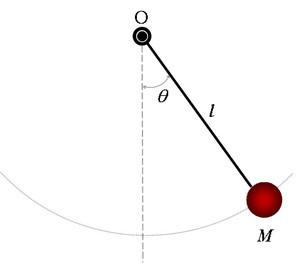
\includegraphics[scale=0.5]{pendulum.jpg}
    \caption{Pendulum}
    \label{fig1}
\end{figure}
Thus the energy $E$ is
\begin{equation}
     E=\frac{1}{2}Ml^2\dot{\theta}^2-Mgl\cos{\theta}.
\end{equation}
We can find the integral for the period
\begin{equation}
    T=4\int_0^{\theta_0}\sqrt{\frac{Ml^2}{2(E+Mgl\cos{\theta})}},
\label{Eq6}
\end{equation}
where $E=-Mgl\cos{\theta_0}$.

If we set
\begin{equation}
    \sin{\eta}=\frac{\sin{\frac{\theta}{2}}}{\sin{\frac{\theta_0}{2}}},
\end{equation}
Eq.(\ref{Eq6}) becomes
\begin{equation}
\begin{aligned}
    T=4\sqrt{\frac{Ml^2}{2(E+Mgl)}}\int_0^{\pi/2}\frac{2\cos\eta\sin{\frac{\theta_0}{2}}}{\sqrt{1-\frac{2Mgl}{E+Mgl}\sin^2{\frac{\theta_0}{2}}\sin^2{\eta}}}\\
    \times\frac{d\eta}{\sqrt{1-\sin^2{\frac{\theta_0}{2}}\sin^2{\eta}}}
\label{Eq7}
\end{aligned}
\end{equation}
Since
\begin{equation}
    \cos{\theta_0}=-\frac{E}{Mgl},
\end{equation}
we have
\begin{equation}
    \sin^2{\theta_0}=\frac{Mgl+E}{2Mgl}.
\end{equation}
Take the above equation into Eq.(\ref{Eq7}), we have
\begin{equation}
\begin{aligned}
    T&=4\sqrt{\frac{l}{g}}\int_0^{\pi/2}\frac{d\eta}{\sqrt{1-\sin^2{\frac{\theta_0}{2}}\sin^2{\eta}}}\\
    &=4\sqrt{\frac{l}{g}}\mathcal{F}(\sin{\frac{\theta_0}{2}}),
\end{aligned}
\end{equation}
where $\mathcal{F}(k)$ is the complete elliptic integral of the first kind.

For some oscillation $\theta_0\rightarrow0$, we have
\begin{equation}
\begin{aligned}
    \int_0^{\pi/2}\frac{d\eta}{\sqrt{1-\sin^2{\frac{\theta_0}{2}}\sin^2{\eta}}}&=\int_0^{\pi/2}(1+\frac{1}{2}\sin^2{\frac{\theta_0}{2}}\sin^2{\eta})d\eta+\mathcal{O}(\theta_0^4)\\
    &=\frac{\pi}{2}+\frac{\sin{\frac{\theta_0}{2}}}{2}\int_0^{\pi/2}\sin^2{\eta}d\eta+\mathcal{O}(\theta_0^4)\\
    &=\frac{\pi}{2}+\frac{\pi}{8}\sin^2{\frac{\theta_0}{2}}+\mathcal{O}(\theta_0^4)
\end{aligned}.
\end{equation}

If we only consider the first order, we finally have
\begin{equation}
    T=2\pi\sqrt{\frac{l}{g}},
\end{equation}
which is our usual approximative period of pendulum.

\subsection{\label{sec:citeref}Tautochrone Problem}
The tautochrone is the curve on which the time of motions under gravity is independent of the initial point. From Part 1 of Section C, we know that, for a tautochrone problem, the potential has quadratic form $U(q)=kq^2$. For motion along a curve $y(x)$, we can use the length $s$ of the arc as the parameter, where $ds^2=dx^2+dy^2$. Then the kinetic energy then becomes
\begin{equation}
    T=\frac{1}{2}m\dot{s}^2.
\end{equation}
And the Lagrangian is
\begin{equation}
\begin{aligned}
    L&=\frac{1}{2}m\dot{s}^2-U(s)
    \\&=\frac{1}{2}m\dot{s}^2-mgy(s)
    \\&=\frac{1}{2}m\dot{s}^2-kmgs^2,
\end{aligned}
\end{equation}
where $y(s)=ks^2$.

Since 
\begin{equation}
    dy=2ks ds,
\end{equation}
and
\begin{equation}
    ds^2=dx^2+dy^2,
\end{equation}
we have
\begin{equation}
dy^2=4k^2s^2(dx^2+dy^2).
\end{equation}
Thus,
\begin{equation}
    (1-4k^2s^2)dy^2=4k^2s^2dx^2.
\end{equation}
By using the function $y(s)=ks^2$, we can get
\begin{equation}
    dx^2=\sqrt{1-4k^2s^2}ds,
\end{equation}
from which we finally get
\begin{equation}
\begin{aligned}
x&=\frac{1}{2}s\sqrt{1-4k^2s^2}+\frac{\arcsin{2ks}}{4k}+const
\\y&=ks^2
\end{aligned}.
\label{Eq8}
\end{equation}

Eq.(\ref{Eq8}) is the parametric function of tautochrone curve in cartesian coordinate.
\begin{figure}
    \centering
    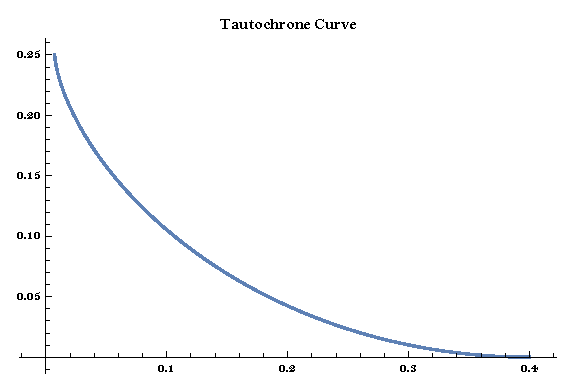
\includegraphics[scale=0.9]{tautochrone.eps}
    \caption{Tautochrone Curve}
    \label{fig2}
\end{figure}
When we choose $const=0.4$,$k=1$,$s\in[-0.5,0]$, we can draw the curve, which is showed in Fig.(\ref{fig2}).







\end{document}

%
% ****** End of file apssamp.tex ******
